% --- I-JEPA Overview ---
\begin{frame}{I-JEPA: Image Joint Embedding Predictive Architecture}
  \begin{itemize}
    \item Introduced by Meta AI (Assran et al., 2023) as an instantiation of Yann LeCun's \textbf{Joint Embedding Predictive Architecture} vision: learn an \emph{internal model} of the world by comparing \textbf{abstract representations} rather than raw pixels.
    \item Self-supervised from unlabeled images; targets are \textbf{feature embeddings} of masked regions predicted from visible context, not pixel reconstruction.
  \end{itemize}
\end{frame}

% --- I-JEPA: Why Predict Features, Not Pixels? ---
\begin{frame}{I-JEPA: Why Predict Features, Not Pixels?}
  \begin{itemize}
    \item Generative objectives often try to explain \textbf{every} missing detail even when the world is \textbf{stochastic} at pixel level, wasting capacity on irrelevant variation (Meta blog example: hands in generative models).
    \item Predicting \textbf{embeddings} steers the model toward \textbf{stable, high-level} structure: objects, parts, and layout.
    \item Empirically: strong \textbf{linear probing} and \textbf{semi-supervised} transfer; competitive on some \textbf{low-level} tasks (e.g.\ counting, depth) despite simpler augmentation than many contrastive methods.
  \end{itemize}
\end{frame}

% --- I-JEPA: Model Architecture ---
\begin{frame}{I-JEPA: Model Architecture (Meta)}
  \begin{columns}[T,onlytextwidth]
    \column{0.5\textwidth}
  \centering
      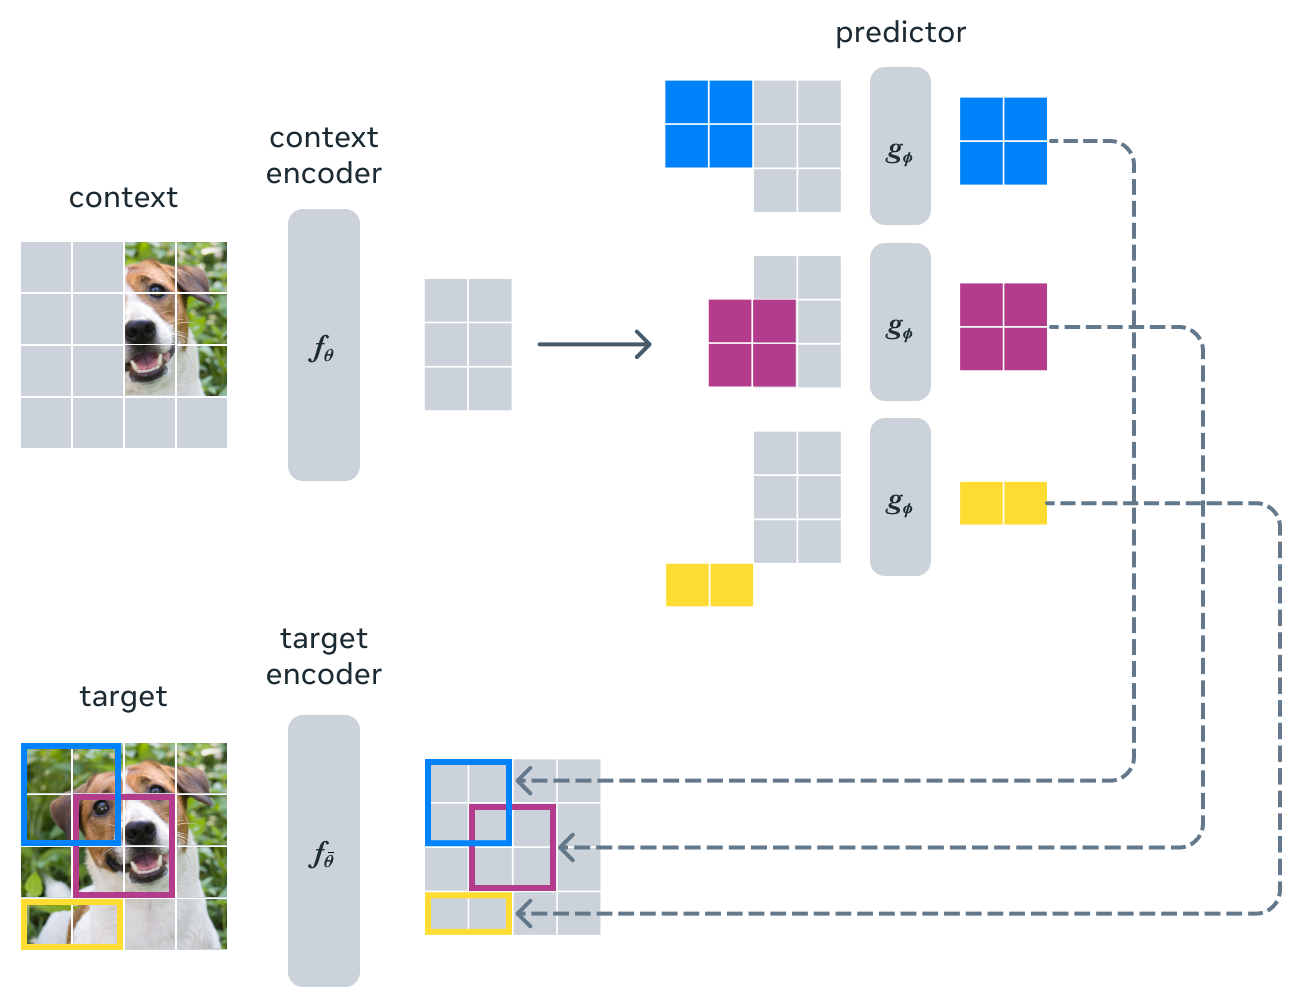
\includegraphics[width=0.95\textwidth, height=0.95\textheight, keepaspectratio]{images/jepa/ijepa_blog_architecture.png}
      {\scriptsize Reference: Meta I-JEPA blog architecture.}
    \column{0.5\textwidth}
  \begin{itemize}
        \item \textbf{Context encoder} ($f_\theta$): ViT on \textbf{visible} patches only.
        \item \textbf{Predictor} ($g_\phi$): narrow ViT that maps context tokens + target \textbf{positional} information to predicted embeddings for each target block.
        \item \textbf{Target encoder} ($f_{\bar{\theta}}$): encodes full image for targets; weights track the context encoder via \textbf{exponential moving average} (EMA), not gradient through targets.
        \item Training minimizes distance between predicted and target \textbf{embeddings}.
  \end{itemize}
  \end{columns}
\end{frame}


% --- I-JEPA: Key Principles ---
\begin{frame}{I-JEPA: Key Principles and Multi-Block Masking}
  \begin{itemize}\itemsep0.28em
    \item SSL objective lives in \textbf{embedding space}: the model predicts \textbf{representations} of target blocks, not pixels.
    \item \textbf{Targets:} sample $M{=}4$ large blocks per image (each $\sim$15--20\% of the image, varied aspect ratio), big enough to carry \textbf{semantic} content, unlike tiny random patches.
    \item \textbf{Context:} one large informative block ($\sim$85--100\% scale) with any overlapping target regions \textbf{removed}, so no target content is visible in the input.
    \item The predictor is a \textbf{restricted world model} for \textbf{static} images: it reasons about what is plausible in unseen regions given partial observation.
    \item Mask design is the \textbf{core inductive bias} of this family; it replaces the hand-crafted augmentations of contrastive methods.
  \end{itemize}
\end{frame}

% --- I-JEPA: Objective and EMA mechanics ---
\begin{frame}{I-JEPA: Objective and EMA Update}
  \textbf{Loss (representation space only):} average $L_2$ distance between predicted and target patch embeddings over the $M$ target blocks $B_i$:
  \begin{equation*}
    \mathcal{L} \;=\; \frac{1}{M}\sum_{i=1}^{M} \;\sum_{j \in B_i} \big\lVert\, \hat{s}_{y}(j) - s_{y}(j) \,\big\rVert_2^2 ,
    \qquad \hat{s}_{y}(j) = g_\phi\!\big(f_\theta(x_{\text{ctx}}),\, m_i\big)
  \end{equation*}
  where $g_\phi$ is the predictor, $f_\theta$ the context encoder, and $m_i$ the target block's \textbf{positional} tokens.
  \vspace{0.4em}
  \begin{itemize}\itemsep0.25em
    \item \textbf{Targets} $s_y(j) = f_{\bar\theta}(y)$ come from the target encoder; \textbf{no gradient} flows through them (stop-gradient).
    \item \textbf{EMA update} of the target encoder (as in BYOL, DINO, and iBOT):
    \begin{equation*}
      \bar\theta \;\leftarrow\; \tau\,\bar\theta + (1-\tau)\,\theta, \qquad \tau \nearrow 1 \text{ over training.}
    \end{equation*}
    \item There are no negatives and no pixel decoder; the asymmetry (predictor + EMA) prevents collapse.
  \end{itemize}
\end{frame}

% --- I-JEPA: Training Dynamics ---
\begin{frame}{I-JEPA: Training and Implementation}
  \begin{itemize}
    \item Sample multi-block masks; for each target block, predict its embedding from context tokens and target position encodings.
    \item \textbf{No multi-view contrastive pipeline:} unlike many SSL methods, I-JEPA avoids expensive pipelines that process many augmented views per step. Only context blocks need the context encoder pass, and the target path uses a single view.
    \item Feature-space loss + EMA target network for stable targets; avoids collapse without pixel reconstruction.
    \item Mask design (large semantic targets, informative context) matters more than hand-crafted view augmentations for this family.
  \end{itemize}
\end{frame}

% --- I-JEPA: Semantic visualization (Meta blog) ---
\begin{frame}{I-JEPA: What Do Predicted Embeddings Encode?}
  \begin{columns}[T,onlytextwidth]
    \column{0.42\textwidth}
    \begin{itemize}\itemsep0.35em
      \item To \textbf{visualize} what the predictor represents, Meta trains a \textbf{stochastic decoder} that maps predicted embeddings toward \textbf{pixel sketches} inside a blue box (for analysis only, not the training objective).
      \item The model tends to capture \textbf{object parts} and \textbf{pose} (e.g.\ dog's head, wolf legs, building structure) rather than arbitrary texture noise.
  \end{itemize}
    \column{0.56\textwidth}
    \centering
    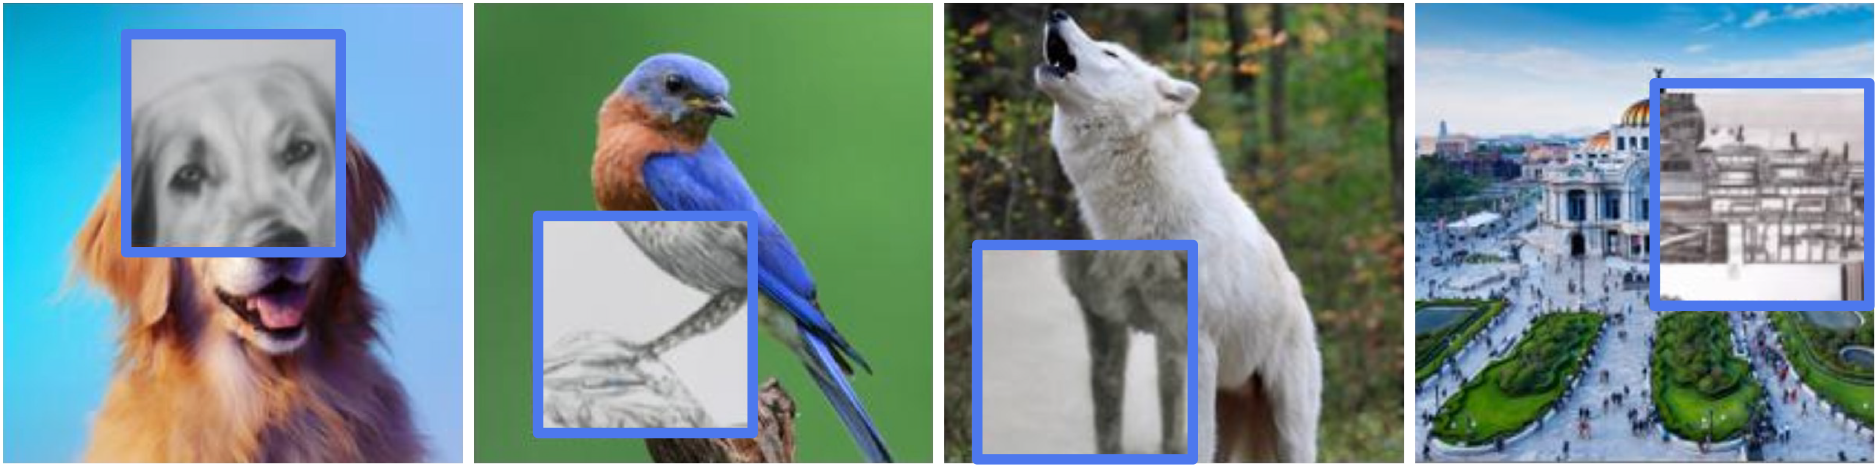
\includegraphics[width=0.95\textwidth, height=0.95\textheight, keepaspectratio]{images/jepa/ijepa_blog_semantic_sketches.png}\\[0.2em]
    {\scriptsize For each image, everything outside the blue box is encoded and given to the predictor as context. A separately trained generative decoder sketches the contents represented by the predictor's output inside the box. The predictor clearly captures the semantics of what should be filled in (the top of the dog's head, the wolf's legs, the other side of the building). Adapted from the Meta I-JEPA blog.}
  \end{columns}
\end{frame}

% --- I-JEPA: Compute efficiency (Meta blog) ---
\begin{frame}{I-JEPA: Compute Efficiency}
  \begin{columns}[T,onlytextwidth]
    \column{0.38\textwidth}
    \begin{itemize}\itemsep0.3em
      \item On ImageNet-1K \textbf{linear evaluation}, I-JEPA reaches strong accuracy at fewer \textbf{pretraining GPU-hours} than several masking and reconstruction baselines (e.g.\ MAE, data2vec) in Meta's reported comparison.
      \item Intuition: representation prediction avoids heavy per-pixel decoder compute and focuses learning on features that transfer.
    \end{itemize}
    \column{0.6\textwidth}
    \centering
    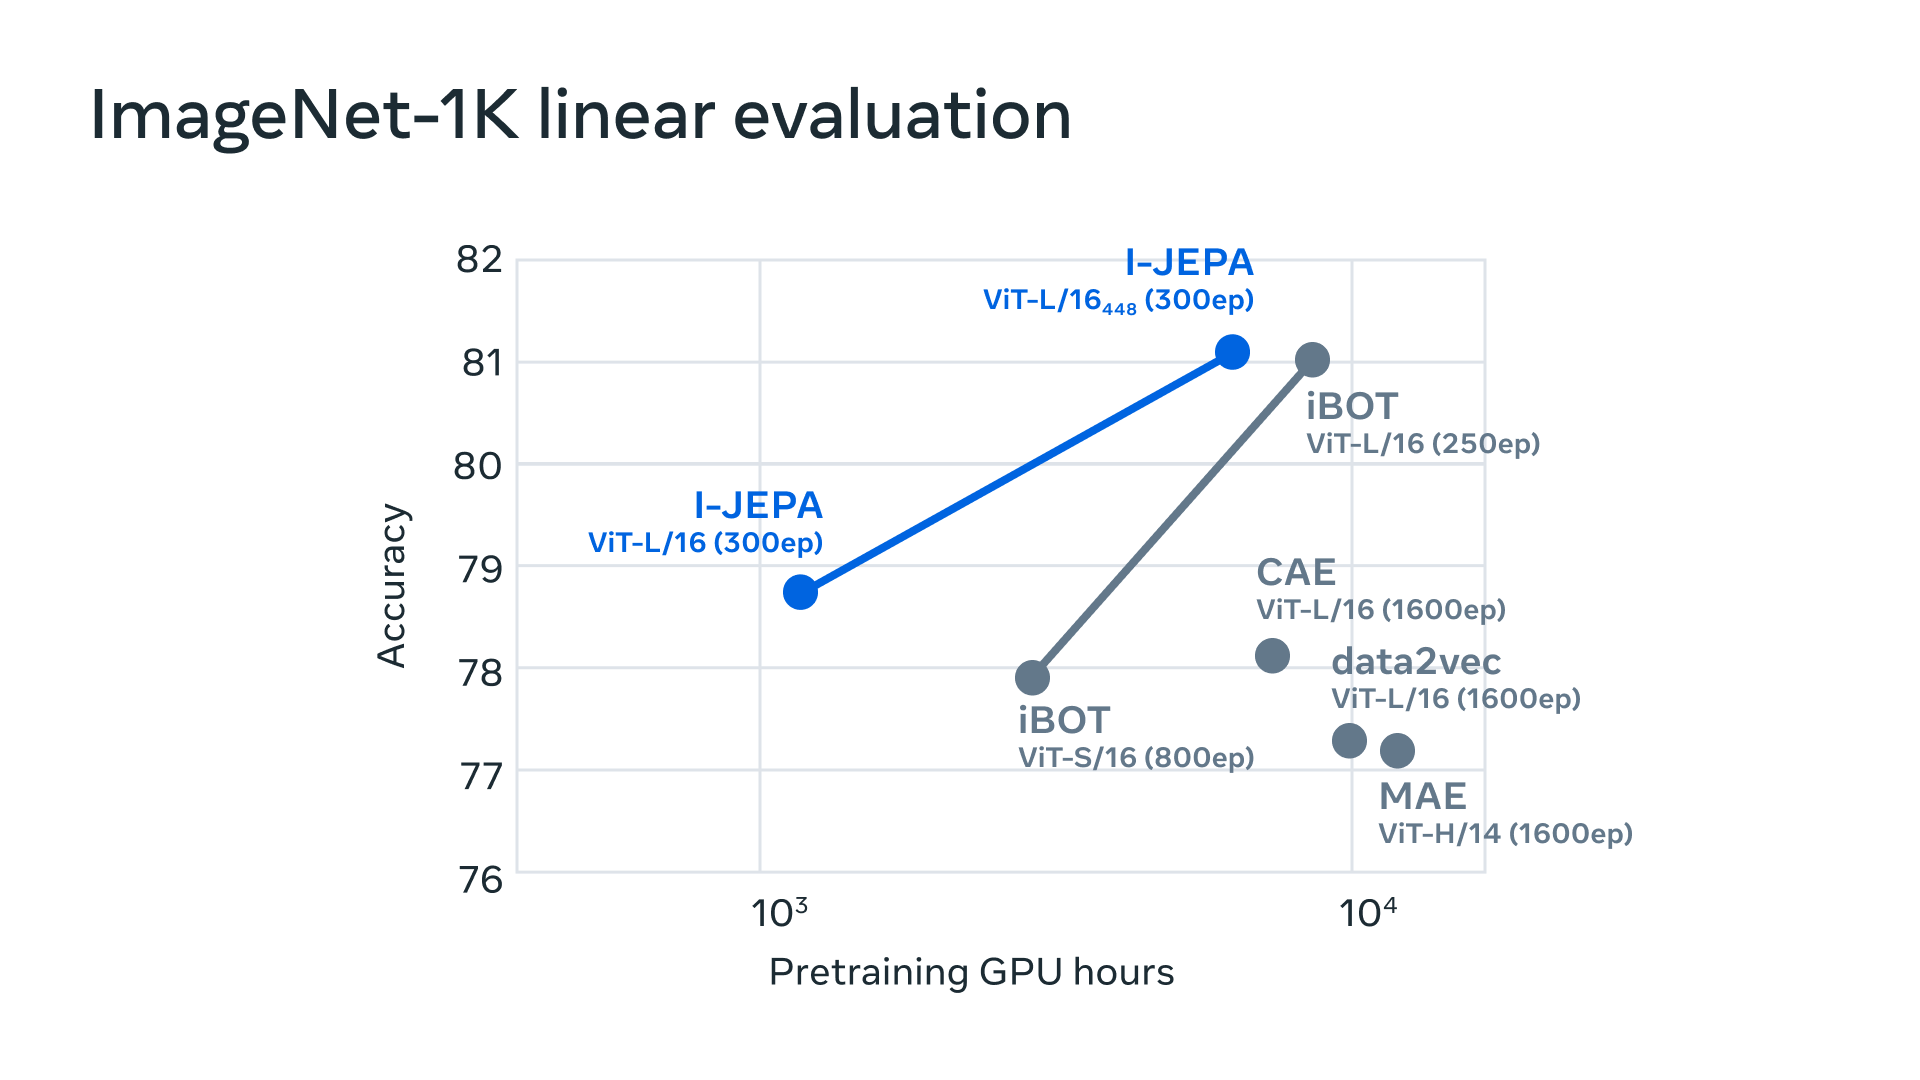
\includegraphics[width=0.8\linewidth, height=0.8\textheight, keepaspectratio]{images/jepa/ijepa_blog_gpu_hours_linear_eval.png}\\[0.2em]
    {\scriptsize ImageNet-1K linear eval vs.\ GPU hours (Meta).}
  \end{columns}
\end{frame}

% --- How SSL encoders are evaluated (protocol primer) ---
\begin{frame}{Evaluating SSL Encoders: Common Protocols}
  \begin{itemize}\itemsep0.25em
    \item \textbf{Frozen evaluation:} pre-trained encoder weights are \textbf{never updated}; only a small head is trained on top. Measures representation quality directly.
    \begin{itemize}\itemsep0.15em
      \item \textbf{Linear probe:} a single linear layer on pooled features.
      \item \textbf{Attentive probe:} a small cross-attention layer pools patch/token features before the classifier. Standard for video models (used by V-JEPA); more expressive than a linear probe but still cheap.
    \end{itemize}
    \item \textbf{Low-shot / semi-supervised:} same idea, but with only e.g.\ 1\%, 5\%, or 10\% of the labels, which tests \textbf{sample efficiency}.
    \item \textbf{Full fine-tuning:} all weights updated on the downstream task. Strongest numbers, but expensive, and no longer a measure of the \emph{pre-trained} representation alone.
    \item JEPA-family papers emphasize \textbf{frozen + low-shot} protocols; keep this in mind when comparing to methods tuned for full fine-tuning (e.g.\ MAE).
  \end{itemize}
\end{frame}

% --- I-JEPA: ImageNet table (Meta blog) ---
\begin{frame}{I-JEPA: Evaluation}
  \centering
  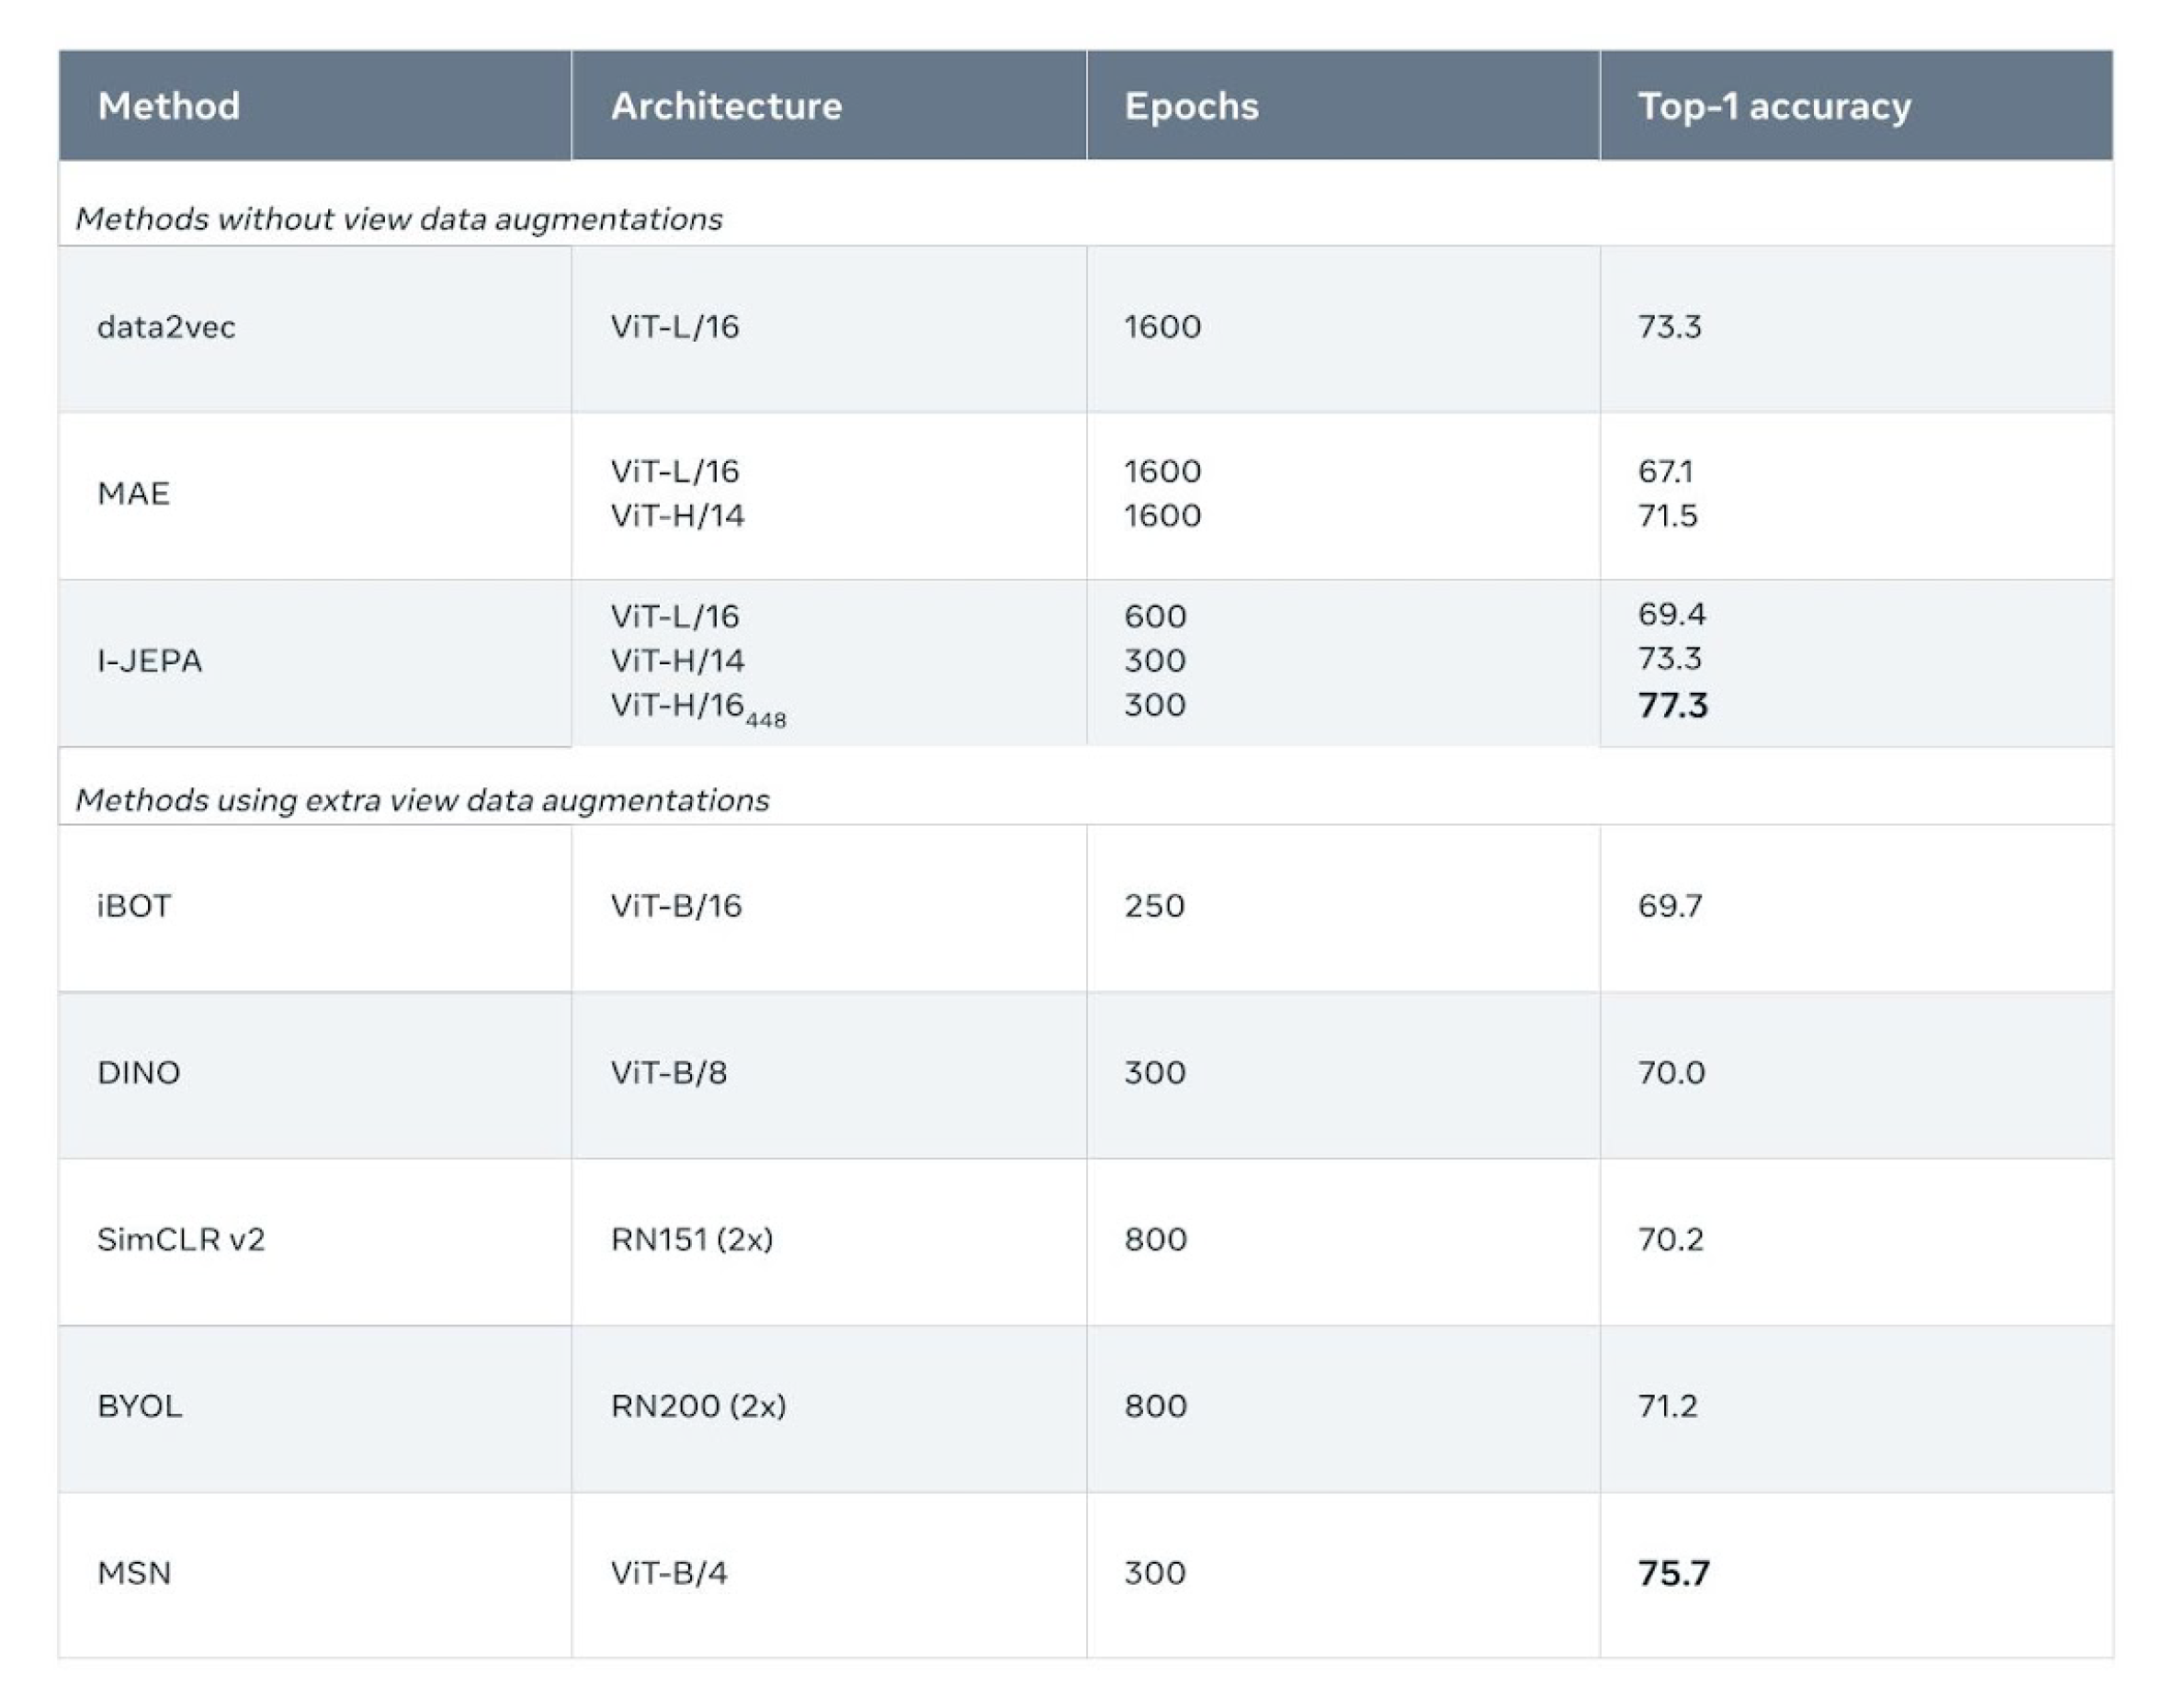
\includegraphics[width=0.8\textwidth, height=0.8\textheight, keepaspectratio]{images/jepa/ijepa_blog_imagenet_linear_table.png}\\[0.35em]
  {\scriptsize Low Shot Classification Accuracy: Semi-supervised evaluation on ImageNet-1k with 1\% of the labels (approximately 12 labeled images per class). Source: \href{https://ai.meta.com/blog/yann-lecun-ai-model-i-jepa/}{Meta I-JEPA blog}, 2023; data from Table~2 of Assran et al., CVPR 2023.}
\end{frame}

% --- I-JEPA: Results and Applications ---
\begin{frame}{I-JEPA: Results and Applications}
  \begin{itemize}
    \item Strong \textbf{off-the-shelf} representations: linear probe, semi-supervised, and competitive low-shot settings without extensive task-specific fine-tuning of the backbone.
    \item Transfers to classification, detection, segmentation-style use cases; blog and paper emphasize \textbf{broader task mix} including some low-level vision tasks.
    \item Open direction: extend JEPAs to \textbf{richer modalities} (video, audio, text conditioning) for longer-horizon \textbf{world models}.
  \end{itemize}
\end{frame}


